\chapter{Equipamentos}

\section{Oculus Rift}

O equipamento é constituído por dois ecrãs OLED, um para cada olho e tem uma resolução de 1080x1200 cada, tem um ângulo de visão de 270 graus, isto cobre praticamente o campo de visão do usuário dando-lhe a máxima experiência do mundo virtual. É também constituído por três giroscópios que capta os movimentos da cabeça do utilizador.

O primeiro protótipo dos Oculus Rift, foi criado em 2009 por Palmer Luckey, este mesmo mais tarde criou uma empresa chamada Oculus que mais tarde em 2014 foi comprada pela empresa Facebook Inc.

Para usar os Oculus Rift é recomendado um computador com capacidades acima das mínimas, pois a realidade virtual requer um pouco das capacidades do computador.

\vspace{5mm}
\begin{figure}[h]
\center
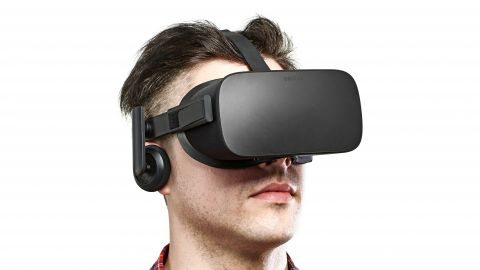
\includegraphics[scale=0.6]{imagens/RV_OR.jpg}
\caption{Exemplo de Oculus Rift. \cite{RV_OR}}
\end{figure}
\vspace{10mm}

\section{Luvas Virtuais}
Luvas virtuais são dispositivos que através de sensores, detetam e medem as flexões e abduções dos dedos, as luvas virtuais na maioria dos casos não são usadas em aplicações sem o apoio de outros equipamentos, ou seja, normalmente pode-se usar juntamente com um fato virtual, um capacete virtual ou os oculus rift. É com a presença destes três equipamentos que obtemos a intitulada realidade virtual.

As luvas virtuais também são usadas no âmbito da medicina (discutida no capitulo anterior). Está a ser testado este equipamento nesta área principalmente para simular operações delicadas, naquelas em que pode não pode haver contacto entre o médico e o paciente pelo risco de morte.


\begin{figure}[h]
\center
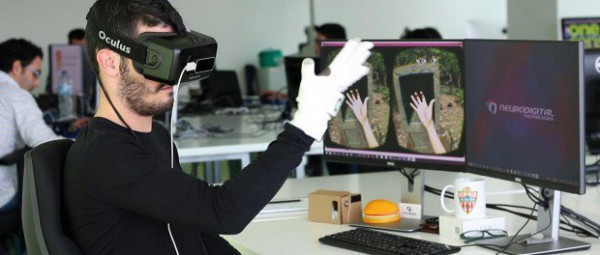
\includegraphics[scale=0.6]{imagens/RV_luvas.jpg}
\caption{Luvas virtuais. \cite{RV_luvas}}
\end{figure}


\section{Icaros}

O Icaros é um simulador que tem como objetivo criar uma sensação de que a pessoa está a flutuar. Utilizando os óculos da realidade virtual juntamente com um aplicativo desenvolvido pelo próprio fabricante, é criado um ambiente praticamente imersivo.

Com ICAROS podemos simular diversas situações desde saltar de uma montanha com paraquedas ou saltar de um avião.

Mas o objetivo do Icaros não é só simular situações de voo, o Icaros também é capaz de simular por exemplo uma moto em alta velocidade, pois o sistema também possui capacidade para tal. No fundo o Icaros é parecido com uma prancha suspensa e possui apoios para os braços e pernas, também é um aparelho para fazer exercício físico, com ele usuário pode treinar diversos grupos musculares, tudo isto dentro da realidade virtual, o usuário poderá fazer exercícios, como subir escadas ou andar de bicicleta. 



\begin{figure}[h]
\center
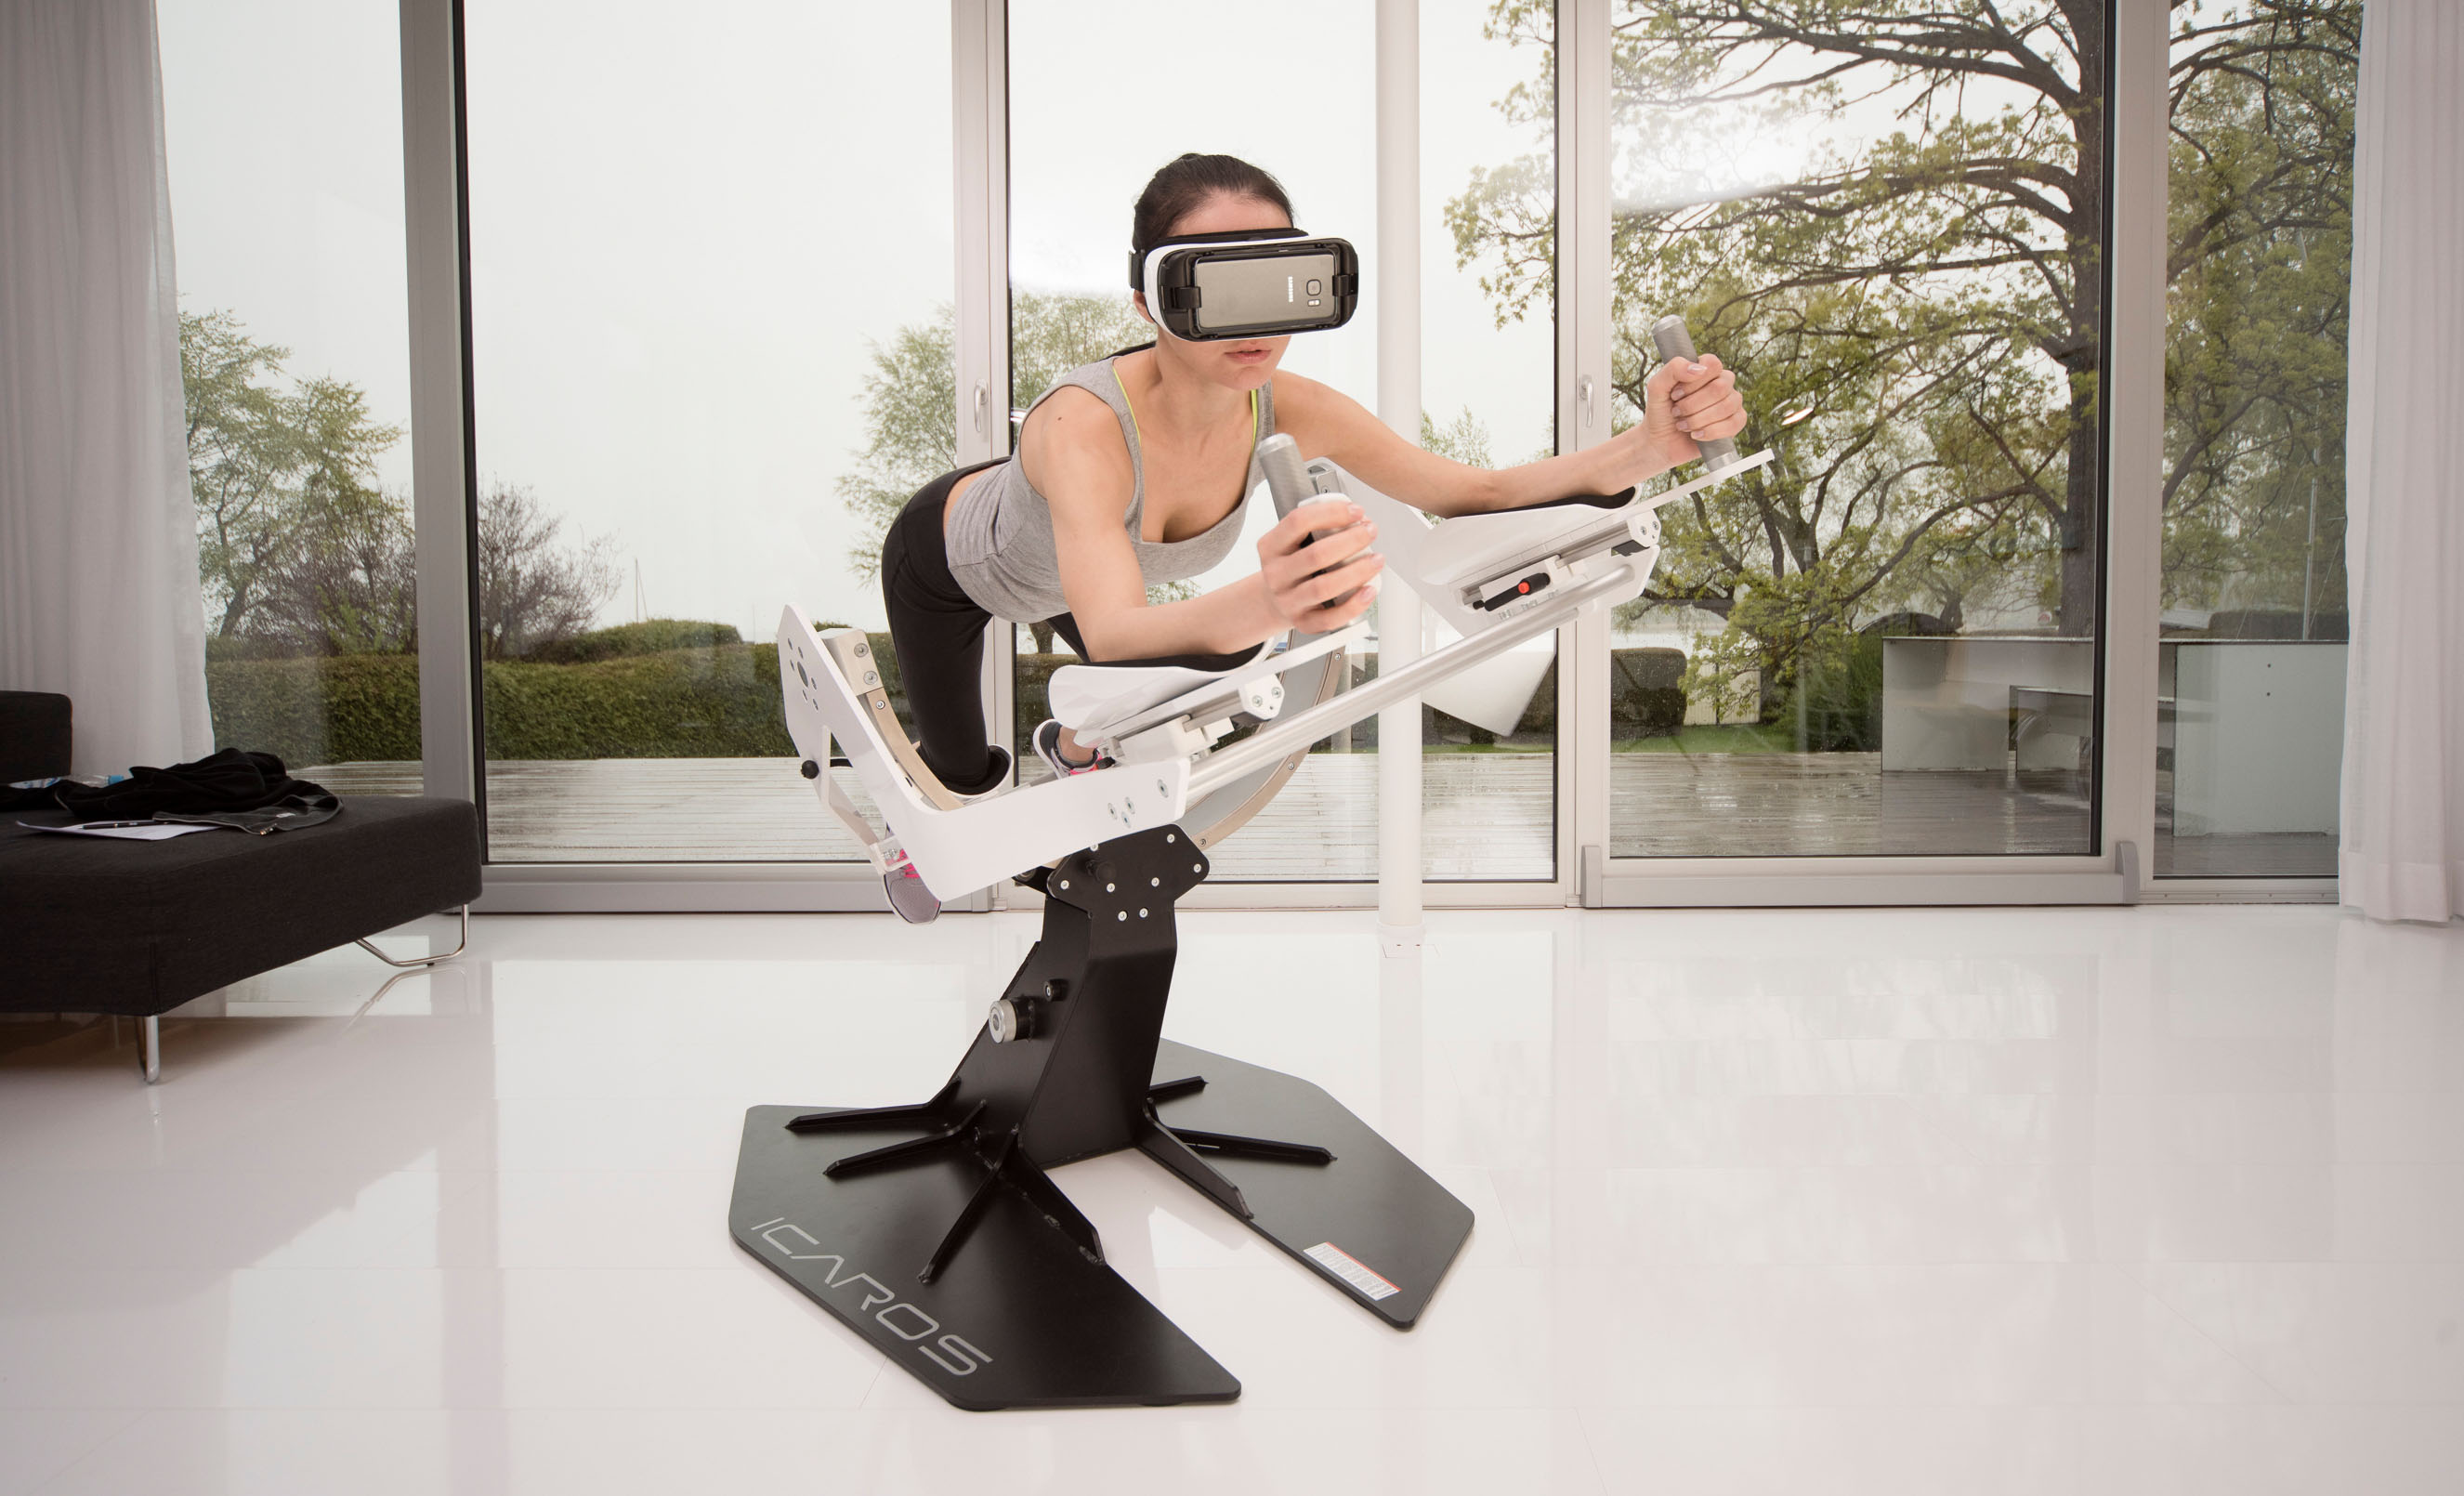
\includegraphics[scale=0.6]{imagens/RV_icaros.jpg}
\caption{Icaros. \cite{RV_icaros}}
\end{figure}


\section{Fato virtual}

Fato virtual Hardlight VR Suit é especialmente desenvolvido para quem é amante de jogos virtuais.

Este fato funciona juntamente com outros equipamentos VR, mas também com jogos de computador comuns.

Este equipamento cobre o tronco e braços por completo e por cada toque que o personagem do jogo sentir o seu usuário no mundo real também sentirá através dos seus 16 sensores espalhados pelo fato que emitem vibrações.


\begin{figure}[H]
\center
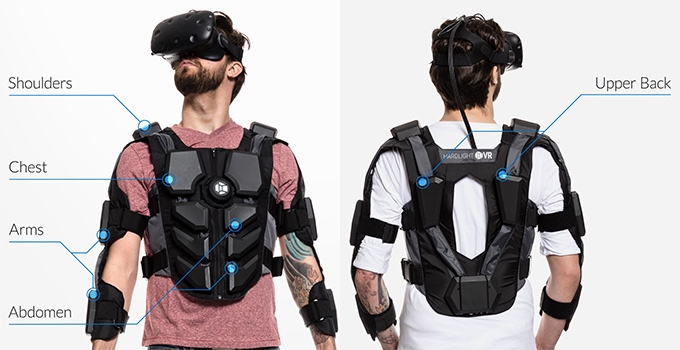
\includegraphics[scale=0.5]{imagens/RV_fato.jpg}
\caption{Fato virtual. \cite{RV_fato}}
\end{figure}



